%!TEX root = ../main.tex

\ParteEsercizi

Ci occuperemo di esperimenti aleatori che ammettono solo un numero \textbf{finito} $n< +\infty $ di risultati possibili. Sia $\Omega =\{\omega_{1} ,\dots ,\omega_{n}\}$ lo spazio campionario associato all'esperimento e $\mathcal{A} =\mathcal{P}(\Omega) =2^{\Omega }$.

Supponiamo che la natura dell'esperimento aleatorio ci suggerisca di assumere $p_{1} =p_{2} =\cdots =p_{n} =p$, i.e. di assegnare la stessa probabilità ad ogni evento elementare. In questo caso si parla di \textbf{spazio di probabilità uniforme}.

\begin{oss}
	In generale non è sempre lecito supporre che la probabilità sia uniforme.
\end{oss}

Dagli assiomi della probabilità segue che:

\begin{equation*}
	1=\PP(\Omega) =\underbrace{\sum\limits_{k=1}^{n}\PP(\{\omega_{k}\}) =\sum\limits_{k=1}^{n} p}_{\text{eventi equiprobabili}} =np=| \Omega | p\implies \boxed{p=\frac{1}{| \Omega | }}
\end{equation*}

Pertanto, quando abbiamo a che fare con esperimenti aleatori su spazi di probabilità uniformi procediamo nel seguente modo:
\begin{enumerate}
	\item individuiamo $\Omega $ (i.e. i possibili esiti dell'esperimento aleatorio) finito, $| \Omega | < +\infty \ \rightarrow \ \mathcal{A} =\mathcal{P}(\Omega) =2^{\Omega }$.
	\item individuiamo il sottoinsieme $A\subseteq \Omega $ che rappresenta l'evento.
	\item se abbiamo probabilità uniforme, cioè gli eventi sono equiprobabili,
	\begin{equation*}
		\boxed{\forall A\in \mathcal{A} \ \ \ \ \PP(A) =\frac{| A| }{| \Omega | } =\frac{\text{casi favorevoli}}{\text{casi possibili}}}
	\end{equation*}
\end{enumerate}
Il problema si riduce sostanzialmente a contare gli elementi di $\Omega $ e di $A$ (i.e. determinare $| \Omega | $ e $|A| $). Per farlo dobbiamo trovare uno \textbf{schema di scelte successive} che ci porti ad individuare univocamente un elemento di $\Omega $ (e di $A$). Questo schema di scelte successive è:
\begin{itemize}
	\item giustificato dal principio fondamentale del calcolo combinatorio;
	\item graficamente visualizzabile tramite un \textbf{diagramma ad albero}.
\end{itemize}
Il calcolo combinatorio è costituito da tecniche che ci permettono di \textbf{contare} il numero di elementi di un insieme \textbf{senza enumerarli} esplicitamente.

\textbf{Principio fondamentale del calcolo combinatorio.} Si realizzano $r$ esperimenti. Si supponga che il primo esperimento abbia $n_{1}$ esiti possibili; che per ognuno di essi il secondo abbia $n_{2} \ $esiti possibili; che per ognuno degli esiti dei primi due esperimenti il terzo esperimento abbia $n_{3}$ esiti possibili ecc. Allora, se sequenze distinte di esiti degli $r$ esperimenti producono esiti finali distinti, allora gli $r$ esperimenti hanno in tutto $n_{1} \cdot n_{2} \cdots n_{r}$ esiti possibili.


\tikzset{every picture/.style={line width=0.75pt}} %set default line width to 0.75pt        

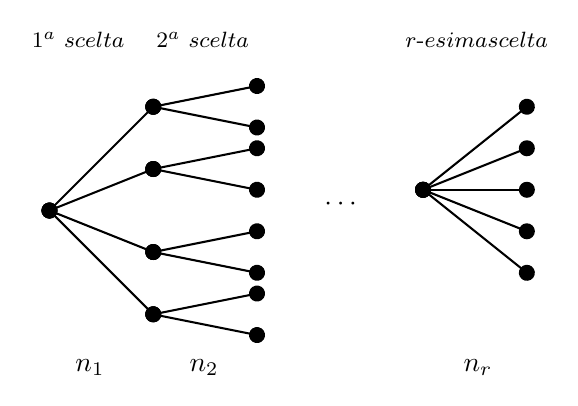
\begin{tikzpicture}[x=0.75pt,y=0.75pt,yscale=-1,xscale=1]
%uncomment if require: \path (0,195); %set diagram left start at 0, and has height of 195

%Straight Lines [id:da7029813942812604] 
\draw    (180,100) -- (230,50) ;
\draw [shift={(230,50)}, rotate = 315] [color={rgb, 255:red, 0; green, 0; blue, 0 }  ][fill={rgb, 255:red, 0; green, 0; blue, 0 }  ][line width=0.75]      (0, 0) circle [x radius= 3.35, y radius= 3.35]   ;
\draw [shift={(180,100)}, rotate = 315] [color={rgb, 255:red, 0; green, 0; blue, 0 }  ][fill={rgb, 255:red, 0; green, 0; blue, 0 }  ][line width=0.75]      (0, 0) circle [x radius= 3.35, y radius= 3.35]   ;
%Straight Lines [id:da3392699638322898] 
\draw    (180,100) -- (230,80) ;
\draw [shift={(230,80)}, rotate = 338.2] [color={rgb, 255:red, 0; green, 0; blue, 0 }  ][fill={rgb, 255:red, 0; green, 0; blue, 0 }  ][line width=0.75]      (0, 0) circle [x radius= 3.35, y radius= 3.35]   ;
\draw [shift={(180,100)}, rotate = 338.2] [color={rgb, 255:red, 0; green, 0; blue, 0 }  ][fill={rgb, 255:red, 0; green, 0; blue, 0 }  ][line width=0.75]      (0, 0) circle [x radius= 3.35, y radius= 3.35]   ;
%Straight Lines [id:da09230469989411372] 
\draw    (180,100) -- (230,150) ;
\draw [shift={(230,150)}, rotate = 45] [color={rgb, 255:red, 0; green, 0; blue, 0 }  ][fill={rgb, 255:red, 0; green, 0; blue, 0 }  ][line width=0.75]      (0, 0) circle [x radius= 3.35, y radius= 3.35]   ;
\draw [shift={(180,100)}, rotate = 45] [color={rgb, 255:red, 0; green, 0; blue, 0 }  ][fill={rgb, 255:red, 0; green, 0; blue, 0 }  ][line width=0.75]      (0, 0) circle [x radius= 3.35, y radius= 3.35]   ;
%Straight Lines [id:da509614192771467] 
\draw    (180,100) -- (230,120) ;
\draw [shift={(230,120)}, rotate = 21.8] [color={rgb, 255:red, 0; green, 0; blue, 0 }  ][fill={rgb, 255:red, 0; green, 0; blue, 0 }  ][line width=0.75]      (0, 0) circle [x radius= 3.35, y radius= 3.35]   ;
\draw [shift={(180,100)}, rotate = 21.8] [color={rgb, 255:red, 0; green, 0; blue, 0 }  ][fill={rgb, 255:red, 0; green, 0; blue, 0 }  ][line width=0.75]      (0, 0) circle [x radius= 3.35, y radius= 3.35]   ;
%Straight Lines [id:da6641758290695727] 
\draw    (230,120) -- (280,110) ;
\draw [shift={(280,110)}, rotate = 348.69] [color={rgb, 255:red, 0; green, 0; blue, 0 }  ][fill={rgb, 255:red, 0; green, 0; blue, 0 }  ][line width=0.75]      (0, 0) circle [x radius= 3.35, y radius= 3.35]   ;
\draw [shift={(230,120)}, rotate = 348.69] [color={rgb, 255:red, 0; green, 0; blue, 0 }  ][fill={rgb, 255:red, 0; green, 0; blue, 0 }  ][line width=0.75]      (0, 0) circle [x radius= 3.35, y radius= 3.35]   ;
%Straight Lines [id:da48211678996199514] 
\draw    (230,120) -- (280,130) ;
\draw [shift={(280,130)}, rotate = 11.31] [color={rgb, 255:red, 0; green, 0; blue, 0 }  ][fill={rgb, 255:red, 0; green, 0; blue, 0 }  ][line width=0.75]      (0, 0) circle [x radius= 3.35, y radius= 3.35]   ;
\draw [shift={(230,120)}, rotate = 11.31] [color={rgb, 255:red, 0; green, 0; blue, 0 }  ][fill={rgb, 255:red, 0; green, 0; blue, 0 }  ][line width=0.75]      (0, 0) circle [x radius= 3.35, y radius= 3.35]   ;
%Straight Lines [id:da8054631564491617] 
\draw    (360,90) -- (410,70) ;
\draw [shift={(410,70)}, rotate = 338.2] [color={rgb, 255:red, 0; green, 0; blue, 0 }  ][fill={rgb, 255:red, 0; green, 0; blue, 0 }  ][line width=0.75]      (0, 0) circle [x radius= 3.35, y radius= 3.35]   ;
\draw [shift={(360,90)}, rotate = 338.2] [color={rgb, 255:red, 0; green, 0; blue, 0 }  ][fill={rgb, 255:red, 0; green, 0; blue, 0 }  ][line width=0.75]      (0, 0) circle [x radius= 3.35, y radius= 3.35]   ;
%Straight Lines [id:da8227041427022426] 
\draw    (360,90) -- (410,110) ;
\draw [shift={(410,110)}, rotate = 21.8] [color={rgb, 255:red, 0; green, 0; blue, 0 }  ][fill={rgb, 255:red, 0; green, 0; blue, 0 }  ][line width=0.75]      (0, 0) circle [x radius= 3.35, y radius= 3.35]   ;
\draw [shift={(360,90)}, rotate = 21.8] [color={rgb, 255:red, 0; green, 0; blue, 0 }  ][fill={rgb, 255:red, 0; green, 0; blue, 0 }  ][line width=0.75]      (0, 0) circle [x radius= 3.35, y radius= 3.35]   ;
%Straight Lines [id:da23191533071565806] 
\draw    (230,80) -- (280,70) ;
\draw [shift={(280,70)}, rotate = 348.69] [color={rgb, 255:red, 0; green, 0; blue, 0 }  ][fill={rgb, 255:red, 0; green, 0; blue, 0 }  ][line width=0.75]      (0, 0) circle [x radius= 3.35, y radius= 3.35]   ;
\draw [shift={(230,80)}, rotate = 348.69] [color={rgb, 255:red, 0; green, 0; blue, 0 }  ][fill={rgb, 255:red, 0; green, 0; blue, 0 }  ][line width=0.75]      (0, 0) circle [x radius= 3.35, y radius= 3.35]   ;
%Straight Lines [id:da015928758957026723] 
\draw    (230,80) -- (280,90) ;
\draw [shift={(280,90)}, rotate = 11.31] [color={rgb, 255:red, 0; green, 0; blue, 0 }  ][fill={rgb, 255:red, 0; green, 0; blue, 0 }  ][line width=0.75]      (0, 0) circle [x radius= 3.35, y radius= 3.35]   ;
\draw [shift={(230,80)}, rotate = 11.31] [color={rgb, 255:red, 0; green, 0; blue, 0 }  ][fill={rgb, 255:red, 0; green, 0; blue, 0 }  ][line width=0.75]      (0, 0) circle [x radius= 3.35, y radius= 3.35]   ;
%Straight Lines [id:da490983698769053] 
\draw    (230,150) -- (280,140) ;
\draw [shift={(280,140)}, rotate = 348.69] [color={rgb, 255:red, 0; green, 0; blue, 0 }  ][fill={rgb, 255:red, 0; green, 0; blue, 0 }  ][line width=0.75]      (0, 0) circle [x radius= 3.35, y radius= 3.35]   ;
\draw [shift={(230,150)}, rotate = 348.69] [color={rgb, 255:red, 0; green, 0; blue, 0 }  ][fill={rgb, 255:red, 0; green, 0; blue, 0 }  ][line width=0.75]      (0, 0) circle [x radius= 3.35, y radius= 3.35]   ;
%Straight Lines [id:da6016628804940389] 
\draw    (230,150) -- (280,160) ;
\draw [shift={(280,160)}, rotate = 11.31] [color={rgb, 255:red, 0; green, 0; blue, 0 }  ][fill={rgb, 255:red, 0; green, 0; blue, 0 }  ][line width=0.75]      (0, 0) circle [x radius= 3.35, y radius= 3.35]   ;
\draw [shift={(230,150)}, rotate = 11.31] [color={rgb, 255:red, 0; green, 0; blue, 0 }  ][fill={rgb, 255:red, 0; green, 0; blue, 0 }  ][line width=0.75]      (0, 0) circle [x radius= 3.35, y radius= 3.35]   ;
%Straight Lines [id:da15071292583890794] 
\draw    (230,50) -- (280,40) ;
\draw [shift={(280,40)}, rotate = 348.69] [color={rgb, 255:red, 0; green, 0; blue, 0 }  ][fill={rgb, 255:red, 0; green, 0; blue, 0 }  ][line width=0.75]      (0, 0) circle [x radius= 3.35, y radius= 3.35]   ;
\draw [shift={(230,50)}, rotate = 348.69] [color={rgb, 255:red, 0; green, 0; blue, 0 }  ][fill={rgb, 255:red, 0; green, 0; blue, 0 }  ][line width=0.75]      (0, 0) circle [x radius= 3.35, y radius= 3.35]   ;
%Straight Lines [id:da4554302375760271] 
\draw    (230,50) -- (280,60) ;
\draw [shift={(280,60)}, rotate = 11.31] [color={rgb, 255:red, 0; green, 0; blue, 0 }  ][fill={rgb, 255:red, 0; green, 0; blue, 0 }  ][line width=0.75]      (0, 0) circle [x radius= 3.35, y radius= 3.35]   ;
\draw [shift={(230,50)}, rotate = 11.31] [color={rgb, 255:red, 0; green, 0; blue, 0 }  ][fill={rgb, 255:red, 0; green, 0; blue, 0 }  ][line width=0.75]      (0, 0) circle [x radius= 3.35, y radius= 3.35]   ;
%Straight Lines [id:da400806931314456] 
\draw    (360,90) -- (410,130) ;
\draw [shift={(410,130)}, rotate = 38.66] [color={rgb, 255:red, 0; green, 0; blue, 0 }  ][fill={rgb, 255:red, 0; green, 0; blue, 0 }  ][line width=0.75]      (0, 0) circle [x radius= 3.35, y radius= 3.35]   ;
\draw [shift={(360,90)}, rotate = 38.66] [color={rgb, 255:red, 0; green, 0; blue, 0 }  ][fill={rgb, 255:red, 0; green, 0; blue, 0 }  ][line width=0.75]      (0, 0) circle [x radius= 3.35, y radius= 3.35]   ;
%Straight Lines [id:da8569851708936509] 
\draw    (360,90) -- (410,90) ;
\draw [shift={(410,90)}, rotate = 0] [color={rgb, 255:red, 0; green, 0; blue, 0 }  ][fill={rgb, 255:red, 0; green, 0; blue, 0 }  ][line width=0.75]      (0, 0) circle [x radius= 3.35, y radius= 3.35]   ;
\draw [shift={(360,90)}, rotate = 0] [color={rgb, 255:red, 0; green, 0; blue, 0 }  ][fill={rgb, 255:red, 0; green, 0; blue, 0 }  ][line width=0.75]      (0, 0) circle [x radius= 3.35, y radius= 3.35]   ;
%Straight Lines [id:da7240053422311326] 
\draw    (360,90) -- (410,50) ;
\draw [shift={(410,50)}, rotate = 321.34] [color={rgb, 255:red, 0; green, 0; blue, 0 }  ][fill={rgb, 255:red, 0; green, 0; blue, 0 }  ][line width=0.75]      (0, 0) circle [x radius= 3.35, y radius= 3.35]   ;
\draw [shift={(360,90)}, rotate = 321.34] [color={rgb, 255:red, 0; green, 0; blue, 0 }  ][fill={rgb, 255:red, 0; green, 0; blue, 0 }  ][line width=0.75]      (0, 0) circle [x radius= 3.35, y radius= 3.35]   ;

% Text Node
\draw (311,92.4) node [anchor=north west][inner sep=0.75pt]    {$\cdots $};
% Text Node
\draw (170,12.4) node [anchor=north west][inner sep=0.75pt]  [font=\footnotesize]  {$1^{a} \ \text{scelta}$};
% Text Node
\draw (230,12.4) node [anchor=north west][inner sep=0.75pt]  [font=\footnotesize]  {$2^{a} \ \text{scelta}$};
% Text Node
\draw (350,12.4) node [anchor=north west][inner sep=0.75pt]  [font=\footnotesize]  {$r\text{\mbox{-}esima scelta}$};
% Text Node
\draw (191,170.4) node [anchor=north west][inner sep=0.75pt]    {$n_{1}$};
% Text Node
\draw (246,170.4) node [anchor=north west][inner sep=0.75pt]    {$n_{2}$};
% Text Node
\draw (378,170.4) node [anchor=north west][inner sep=0.75pt]    {$n_{r}$};


\end{tikzpicture}

\begin{oss}
	Il diagramma ad albero è utile per rappresentare tutti i casi possibili: ci permette di avere un'elencazione grafica di tutti gli elementi di $\Omega $ (e/o di $A\in \mathcal{A}$).
\end{oss}

\begin{oss}
	Lo schema di scelte successive deve individuare univocamente gli elementi degli insiemi (come da principio).
\end{oss}

\textbf{Permutazioni, disposizioni e combinazioni.}

Sono concetti utili per contare gli elementi in un insieme.

\begin{definition}
	Le permutazioni di $n$ oggetti sono tutti i possibili ordinamenti di $n$ oggetti. Le permutazioni di $n$ oggetti sono pari a:
	\begin{equation*}
		\boxed{P_{n} =n!=n(n-1)(n-2) \cdots 1} \ \ \ \ (0!\coloneqq 1)
	\end{equation*}
	Ho $n$ scelte per il primo oggetto, $(n-1)$ scelte per il secondo ecc.
\end{definition}

\begin{oss}
	Vi sono
	\begin{equation*}
		\boxed{P_{n}^{n_{1} ,n_{2} ,\dots ,n_{r}} =\frac{n!}{n_{1} !\ n_{2} !\cdots n_{r} !}}
	\end{equation*}
	permutazioni di un insieme di $n$ oggetti, dei quali $n_{1}$ sono identici tra loro, $n_{2}$ sono identici tra loro e distinti dai precedenti, $\dots $, $n_{r}$ sono identici e distinti dai precedenti.
\end{oss}

\textit{Esempio.} Classifica di $n$ persone, ci sono $n!$ possibili ordinamenti delle persone.

Supponiamo di avere un insieme $E$ formato da $n$ oggetti \textbf{distinti}, da cui ne estraiamo $r$.
\begin{definition}
	Le \textbf{disposizioni con ripetizione di classe }$r$ sono le stringhe di $r$ elementi di $E$. Il modello è quello dell'\textit{estrazione con reimmissione} da un'urna contenente $n$ oggetti. Ogni volta lo rimetto nell'urna. Ogni volta ho $n$ modi di scegliere:
	\begin{equation*}
		\boxed{D'^{n}_{r} =\underbrace{n\cdot n\cdots n}_{r\ \text{volte}} =n^{r}}
	\end{equation*}
\end{definition}

\begin{definition}
	Le \textbf{disposizioni senza ripetizione di classe} $r$ sono le $r$-ple ordinate di elementi di $E$ senza ripetizione (deve essere $r\leq n$). Il modello è quello dell'\textit{estrazione senza reimmissione} da un'urna contenente $n$ oggetti. Ogni volta ho un modo in meno di scegliere. \textit{L'ordine conta}.
	\begin{equation*}
		\boxed{D_{r}^{n} =n(n-1)(n-2) \cdots (n-r+1) =\frac{n!}{(n-r) !}}
	\end{equation*}
\end{definition}

\begin{oss}
	Le permutazioni sono un caso particolare di disposizioni senza ripetizione: $n!=D_{n}^{n}$.
\end{oss}

\textit{Esempio.} I primi $r$ classificati in una gara di $n$ persone.

\begin{definition}
	Ogni sottoinsieme di $E$ di cardinalità $r\leq n$ è detto \textbf{combinazione di classe} $r$ di $E$. Il modello è quello di un'\textit{estrazione simultanea} di $r$ oggetti da un'urna che ne contiene $n$ $(r\leq n)$. Simile alle disposizioni, ma qui \textit{l'ordine non conta}.
	\begin{equation*}
		\boxed{C_{r}^{n} =\binom{n}{r} =\frac{n!}{r!(n-r) !}}
	\end{equation*}
\end{definition}

\begin{oss}
Per determinare $C_{r}^{n}$ basta osservare che: ogni fissata combinazione di classe $r$ dà luogo a $r!$ disposizioni di classe $r$, i.e. ho $r!$ possibili modi di permutare gli oggetti:
	\begin{equation*}
		D_{r}^{n} =r!\ C_{r}^{n}
	\end{equation*}
	Ora,
	\begin{equation*}
		D_{r}^{n} =n(n-1) \cdots (n-r+1) =\frac{n!}{(n-r) !}
	\end{equation*}
	Quindi:
	\begin{equation*}
		r!\ C_{r}^{n} =\frac{n!}{(n-r) !} \implies C_{r}^{n} =\frac{n!}{r!(n-r) !} =\binom{n}{r}
	\end{equation*}
\end{oss}

\Esercizio{}

Lanciate due volte un dado non truccato.
\begin{enumerate}
	\item Qual è la probabilità di un $6$ al primo lancio?
	\item Qual è la probabilità che la somma dei due risultati dia un $6$?
	\item A quanto è pari quest'ultima probabilità se lanciate tre volte il dado?
\end{enumerate}

\Esercizio{}

Trovate una ventiquattrore chiusa con combinazione di $6$ cifre. Con quale probabilità riuscirete ad aprirla al primo tentativo? E se la combinazione fosse di $6$ lettere scelte fra $A$, $B$, $C$ e $D$?

\Esercizio{}

Scommetto sui primi $5$ classificati di una gara con $40$ concorrenti, senza conoscerli.
\begin{enumerate}
	\item Qual è la probabilità di vincere?
	\item E se scommettessi sui nomi dei primi cinque, senza precisarne l'ordine?
\end{enumerate}

\Esercizio{(Paradosso dei compleanni)}

\begin{enumerate}
	\item Qual è la probabilità $p_{n}$ che, in un gruppo di $n$ persone selezionate in modo casuale (nate tutte in un anno non bisestile), almeno due di esse compiano gli anni lo stesso giorno? Quanto deve essere grande $n$ affinché $p_{n}  >\frac{1}{2}$?
	\item Qual è la probabilità $q_{n}$ che, nel gruppo di $n$ persone, ve ne sia almeno una che compie gli anni il vostro stesso giorno (posto che non siate nati il 29 febbraio)?Quanto deve essere grande $n$ affinché $q_{n}  >\frac{1}{2}$?
\end{enumerate}

\Esercizio{}

Tre amici si danno appuntamento nel bar della piazza centrale della città senza sapere che ci sono quattro bar. Qual è la probabilità che scelgano lo stesso bar? Tre bar differenti?

\Esercizio{}

Confrontate la probabilità di ottenere almeno un $6$ nel lancio di $6$ dadi con la probabilità di ottenere almeno due $6$ nel lancio di $12$ dadi.

\Esercizio{}

Una moneta viene lanciata $4$ volte. Quali sono le probabilità di ottenere $3$ teste e una croce e di ottenere $2$ teste e $2$ croci?

\Esercizio{}

Per compilare una colonna di una schedina del Totocalcio occorre scegliere, per ciascuna delle $13$ partite in esame, tra la vittoria della squadra di casa $(1)$, il pareggio $(X)$ o la vittoria della squadra in trasferta $(2)$. Si calcoli la probabilità di fare $13$ o $12$ al Totocalcio giocando per ogni partita una doppia (due possibili risultati per ogni partita). Si suppongano equiprobabili le possibili schedine.

\Esercizio{}

Giocate $6$ numeri al Superenalotto. Saranno estratti $6$ numeri senza ripetizione dai primi $90$ naturali, seguiti dall'estrazione di un $7^{o}$ numero jolly, diverso quindi dai precedenti. Qual è la probabilità di fare
\begin{enumerate}
	\item $6$ (indovinare i primi $6$ numeri estratti)?
	\item $5+1$ (indovinare $5$ dei primi $6$ numeri estratti e in più il numero jolly)?
	\item $6$ o $5+1$?
\end{enumerate}

Quale o quali spazi campionari avete introdotto per rispondere ai punti precedenti? Sono scelte coerenti?

\Esercizio{}

Si consideri l'estrazione di $k$ oggetti da un'urna contenente $n$ oggetti distinti, numerati da $1$ a $n$.
\begin{enumerate}

	\item Si consideri l'estrazione con reimmissione, per cui $k\in \NN$. Viene osservato il risultato ordinato delle $k$ estrazioni.
	\begin{enumerate}
		\item Individuare il più piccolo spazio campionario $\Omega $ che permette di descrivere l'esperimento aleatorio.
		\item * Dimostrare che i possibili risultati dell'esperimento aleatorio sono equiprobabili se e solo se le $k$ estrazioni sono indipendenti e per ciascuna singola estrazione gli $n$ possibili risultati sono equiprobabili.
		\item Calcolare la probabilità di estrarre un dato insieme di oggetti $\{x_{1} ,\dots ,x_{k}\}$, senza riguardo per l'ordine di estrazione.
	\end{enumerate}

	\item Si consideri l'estrazione senza reimmissione, per cui $1\leq k\leq n$. Viene osservato il risultato ordinato delle $k$ estrazioni.
	\begin{enumerate}
		\item Individuare il più piccolo spazio campionario $\Omega $ che permette di descrivere l'esperimento aleatorio.
		\item * Dimostrare che i possibili risultati dell'esperimento aleatorio sono equiprobabili se e solo se il risultato di ciascuna delle $k$ estrazioni, data la sequenza degli oggetti già estratti, è equiprobabile fra gli oggetti rimanenti.
		\item Calcolare la probabilità di estrarre un dato insieme di oggetti $\{x_{1} ,\dots ,x_{k}\}$, senza riguardo per l'ordine di estrazione.
	\end{enumerate}

	\item Si consideri l'estrazione simultanea, per cui $1\leq k\leq n$. Viene osservato il risultato dell'estrazione.
	\begin{enumerate}
		\item Individuare il più piccolo spazio campionario $\Omega $ che permette di descrivere l'esperimento aleatorio.
		\item Calcolare la probabilità di estrarre un dato insieme di oggetti $\{x_{1} ,\dots ,x_{k}\}$.
	\end{enumerate}

\end{enumerate}

\Esercizio{}

Si calcoli la probabilità di ottenere $2$ palline rosse estraendone $4$ da un'urna che contiene $3$ palline rosse e $7$ bianche. Si confrontino i casi di estrazioni con reimmissione, senza reimmissione e simultanea.

\Esercizio{}

Si estraggono, con o senza reimmissione, $7$ palline da un'urna contenente $4$ palline bianche e $8$ rosse. Qual è la probabilità di estrarne esattamente $3$ bianche?

\Esercizio{}

Da un'urna contenente $5$ palline bianche, $7$ rosse e $4$ blu, vengono estratte senza reimmissione $5$ palline. Con quale probabilità si ottengono $3$ bianche, $1$ rossa e $1$ blu?

\Esercizio{}

Si estraggono $2$ palline da un'urna contenente $5$ palline bianche, $6$ nere e $4$ rosse. Calcolare la probabilità che siano dello stesso colore. Distinguere il caso di estrazione simultanea o con reimmissione.

\Esercizio{}

Si consideri l'estrazione di $n$ palline da un'urna contenente $B$ palline bianche e $R$ palline rosse. Qual è la probabilità di estrarne esattamente $k$ rosse, con $0\leq k\leq n$? Si risponda nel caso di estrazione con reimmissione e nel caso di estrazione simultanea.

\Esercizio{}

A scommette con B che estrarrà 4 carte di 4 semi diversi da un mazzo di 40 carte. Qual è la probabilità che A vinca?

\Esercizio{}

Supponiamo di giocare a poker con un mazzo da $52$ carte, identificate dal seme (cuori $\varheartsuit $, quadri $\vardiamondsuit $, fiori $\clubsuit $, picche $\spadesuit $) e dal tipo (un numero da $2$ a $10$ oppure $J$, $Q$, $K$, $A$). Si calcolino:
\begin{enumerate}
	\item la probabilità di avere un full, ovvero un sottoinsieme di $5$ carte $\{X_{1} ,X_{2} ,X_{3} ,Y_{1} ,Y_{2}\}$ costituito dall'unione di un tris (un sottoinsieme di $3$ carte $X_{1} ,X_{2} ,X_{3}$ dello stesso tipo) e di una coppia (un sottoinsieme di $2$ carte $Y_{1} ,Y_{2}$ dello stesso tipo);
	\item la probabilità di avere una doppia coppia, ovvero un sottoinsieme di $5$ carte $\{X_{1} ,X_{2} ,Y_{1} ,Y_{2} ,Z\}$ costituito dall'unione di due coppie $\{X_{1} ,X_{2}\}$, $\{Y_{1} ,Y_{2}\}$ di tipi diversi, più una quinta carta $Z$ di tipo diverso dai tipi delle due coppie;
	\item la probabilità di avere una scala reale massima, ovvero le $5$ carte $10,J,Q,K,A$ dello stesso seme;
	\item la probabilità di avere una scala reale, ovvero una qualsiasi scala di $5$ carte dello stesso seme (ricordiamo che con l'asso possiamo fare la scala $A,2,3,4,5$ ma anche $10,J,Q,K,A$);
	\item la probabilità di avere una scala, ovvero una qualsiasi scala di $5$ carte non necessariamente dello stesso seme;
	\item la probabilità di avere colore, ovvero un sottoinsieme di $5$ carte dello stesso seme;
	\item la probabilità di avere poker, ovvero un sottoinsieme di $5$ carte in cui ci sono $4$ carte dello stesso tipo;
	\item la probabilità di avere un tris, ovvero un sottoinsieme di $5$ carte in cui ci sono $3$ carte dello stesso tipo e le altre due di tipo diverso tra loro e dalle prime tre;
	\item la probabilità di avere una coppia, ovvero un sottoinsieme di $5$ carte in cui ci sono $2$ carte dello stesso tipo e le altre tre di tipo diverso tra loro e dalle prime due.
\end{enumerate}

\Esercizio{}

Un mazzo di carte da scopone scientifico è costituito da $40$ carte, identificate dal seme (spade, coppe, bastoni, denari) e dal tipo (asso, $2$, $3$, $4$, $5$, $6$, $7$, fante, cavallo, re). Supponendo di pescare $10$ carte dal mazzo, calcolare la probabilità di estrarre:
\begin{enumerate}
	\item l'asso di bastoni,
	\item l'asso di spade e l'asso di coppe,
	\item almeno un asso fra l'asso di spade e l'asso di coppe.
\end{enumerate}

\Esercizio{}

Facendo uso del calcolo combinatorio, dimostrare che
\begin{equation*}
	(a+b)^{n} =\sum\limits_{k=0}^{n}\binom{n}{k} a^{k} b^{n-k}
\end{equation*}

\Esercizio{}

Dato un insieme finito $\Omega $ di cardinalità $| \Omega | $, dimostrare che il suo insieme delle parti $\mathcal{P}(\Omega) =2^{\Omega }$ ha cardinalità $2^{| \Omega | }$.

\ParteSoluzioni

\Soluzione

\begin{enumerate}
	\item Lo spazio degli eventi elementari è
	\begin{gather*}
		\Omega =\{(i,j) :i,j=1,\dots ,6\} =\{1,\dots ,6\}^{2} ,\ \ \ \ | \Omega | =36\\
		i=\text{primo lancio} \ \ \ \ j=\text{secondo lancio}
	\end{gather*}
	Come famiglia ($\sigma $-algebra) degli eventi possibili possiamo scegliere $\mathcal{A} \coloneqq \mathcal{P}(\Omega) =2^{\Omega }$. Per quanto riguarda l'assegnazione di una probabilità $\PP$ su $(\Omega ,\mathcal{A})$ osserviamo che se assumiamo che i due non siano truccati e vogliamo che il nostro spazio di probabilità $(\Omega ,\mathcal{A} ,\PP)$ modellizzi questo fatto fisico, dobbiamo ammettere che tutti gli eventi elementari di $\Omega $ abbiano la stessa probabilità $\PP =\frac{1}{| \Omega | } =\frac{1}{36}$. Siamo pertanto in uno spazio campionario con probabilità uniforme. Allora $\forall A\in \mathcal{A} ,\PP(A) =\frac{| A| }{| \Omega | } =\frac{| A| }{36}$.

	Sia $A$ l'evento "avere un $6$ al primo lancio", allora
	\begin{gather*}
		A=\{(6,1) ,(6,2) ,(6,3)(6,4) ,(6,5) ,(6,6)\} ,\ \ \ \ | A| =6\\
		\implies \PP(A) =\frac{| A| }{| \Omega | } =\frac{6}{36} =\frac{1}{6} \approx 0.1667
	\end{gather*}

	\begin{oss}
		In questo caso $\Omega $ ed $A$ hanno pochi elementi e possiamo elencarli senza problemi. Avremmo anche potuto contare gli elementi di $A$ e $\Omega $ senza elencarli con un diagramma ad albero.
	\end{oss}

	\item Sia $B$ l'evento "la somma dei due risultati è $6$", allora
	\begin{gather*}
		B=\{(5,1) ,(2,4) ,(3,3) ,(4,2) ,(1,5)\} ,\ \ \ \ | B| =5\\
		\implies \PP(B) =\frac{| B| }{| \Omega | } =\frac{5}{36} \approx 0.1389
	\end{gather*}

	\begin{oss}
		I risultati della somma non sono equiprobabili. Infatti, se assumiamo che i due dadi non siano truccati, denotando con $\{i\}$ l'evento "la somma dei due dadi è $i$", per $i=1,\dots ,12$,
		\begin{equation*}
			\begin{array}{ l }
				\PP(\{2\}) =\PP(\{12\}) =1/36\\
				\PP(\{3\}) =\PP(\{11\}) =1/18\\
				\PP(\{4\}) =\PP(\{10\}) =1/12\\
				\PP(\{5\}) =\PP(\{9\}) =1/9\\
				\PP(\{6\}) =\PP(\{8\}) =5/36\\
				\PP(\{7\}) =1/6
			\end{array}
		\end{equation*}
		Se invece assumiamo che i possibili risultati della somma siano equiprobabili, dobbiamo porre
		\begin{equation*}
			\PP(\{i\}) =\frac{1}{11} \ \ \ \ 11=| \Omega | \ \text{con} \ \Omega =\{2,3,\dots ,12\}
		\end{equation*}
		$\Omega =$ spazio degli eventi elementari, somma degli esiti del lancio dei due dadi. Lo spazio di probabilità così costruito è matematicamente corretto, ma non ha nulla a che fare con la realtà fisica dell'esperimento.
	\end{oss}

	\item Lanciando $3$ volte il dado lo spazio campionario diventa
	\begin{equation*}
		\Omega =\{(i,j,k) :i,j,k=1,\dots ,6\} =\{1,\dots ,6\}^{3} \ \ \ \ | \Omega | =6^{3} =216
	\end{equation*}

	Sia $C$ l'evento "la somma dei dadi è $6$"
	\begin{gather*}
		\begin{aligned}
			C= & (\{1,1,4\} ,\{1,4,1\} ,\{4,1,1\} ,\\
			 & \{1,2,3\} ,\{1,3,2\} ,\{2,1,3\} ,\{2,3,1\} ,\{3,1,2\} ,\{3,2,1\} ,\\
			 & \{2,2,2\})
		\end{aligned}\\
		\implies \PP(C) =\frac{| C| }{| \Omega | } =\frac{10}{6^{3}} \approx 0.0463
	\end{gather*}

	\begin{oss}
		Avremmo potuto risolvere l'esercizio anche sfruttando il concetto di permutazioni, definendo
		\begin{gather*}
			C=\text{possibili permutazioni di} \ 
			\begin{cases}
				\{1,2,3\} & \rightarrow 3!=6\ \text{permutazioni}\\
				\{2,2,2\} & \rightarrow 1\ \text{permutazione}\\
				\{1,1,4\} & \rightarrow 3!/2!=3\ \text{permutazioni}
			\end{cases}\\
			\implies | C| =6+3+1=10
		\end{gather*}
	\end{oss}
	
\end{enumerate}

\Soluzione

Manca.

\Soluzione

Consideriamo i due eventi
\begin{itemize}
	\item $A=$ \event{vinco}, i.e. azzecco la cinquina vincente
	\item $B=$ \event{vinco senza precisare l'ordine}
\end{itemize}

Svolgiamo l'esercizio in $3$ diversi modi.

\textbf{[Metodo 1]}

Determiniamo innanzitutto l'insieme campionario $\Omega $: c'è una classifica di cui ci interessano solo i primi $5$:
\begin{equation*}
	\Omega =\{(\omega_{1} ,\dots ,\omega_{5}) :\omega_{i} \in \{1,\dots,40\} ,\omega_{i} \neq \omega_{j} \ \forall i\neq j\}
\end{equation*}
Tutte le possibili quintuple sono date dalla disposizione (l'ordine conta!) di $n=40$ persone in $r=5$ posti, i.e.
\begin{equation*}
	| \Omega | =D_{5}^{40} =\underbrace{40\cdot 39\cdots 36}_{5\ \text{numeri}} =78960960
\end{equation*}
Per il primo ci sono $40$ possibilità, per il secondo $39$, ecc. (visualizzabile con un diagramma ad albero.
\begin{enumerate}
	\item Ho esattamente $1$ possibilità (su tutte quelle possibili) di vincere.
	\begin{equation*}
		| A| =1\implies \PP(A) =| A| /| \Omega | =1/78960960\approx 1.3\times 10^{-8}
	\end{equation*}
	\item Se non preciso l'ordine ho $5!$ modi di scegliere la cinquina vincente, i.e. tutte le $5!$ permutazioni dei primi $5$ classificati.
	\begin{equation*}
		| B| =5!\implies \PP(B) =| B| /| \Omega | =5!/78960960\approx 1.5\times 10^{-6}
	\end{equation*}
\end{enumerate}

\textbf{[Metodo 2]}

Guardiamo tutta la classifica. In questo caso dobbiamo considerare le permutazioni di $40$ oggetti:
\begin{equation*}
	\Omega =\{(\omega_{1} ,\dots ,\omega_{40}) :\omega_{i} \in \{1,\dots,40\} ,\omega_{i} \neq \omega_{j} \ \forall i\neq j\} \ \ \ \ | \Omega | =40!
\end{equation*}
\begin{enumerate}
	\item Evento $A$.
	\begin{center}
	\addstackgap[5pt]{
		\begin{tabular}{cc|c}
			\hline 
			scelgo il numero $1$: & $1$ modo & \multirow{3}{*}{$1$ permutazione} \\
			$\vdots $ & $\vdots $ &   \\
			scelgo il numero $5$: & $1$ modo &   \\
			\hline 
			scelgo il numero $6$: & $35$ modi & \multirow{4}{*}{$35!$ permutazioni} \\
			scelgo il numero $7$: & $34$ modi &   \\
			$\vdots $ & $\vdots $ &   \\
			scelgo il numero $40$: & $1$ modo &   \\
			\hline
		\end{tabular}
		}
	\end{center}
	i.e. $| A| =35!\implies \PP(A) =| A| /| \Omega | =35!/40!\approx 1.3\times 10^{-8}$.
	\item Evento $B$. Simile a prima, ma abbiamo $5!$ modi di scegliere i primi $5$ arrivati:
	\begin{center}
	\addstackgap[5pt]{
		\begin{tabular}{cc|c}
			\hline 
			scelgo il numero $1$: & $5$ modi & \multirow{3}{*}{$5!$ permutazioni} \\
			$\vdots $ & $\vdots $ &   \\
			scelgo il numero $5$: & $1$ modo &   \\
			\hline 
			scelgo il numero $6$: & $35$ modi & \multirow{4}{*}{$35!$ permutazioni} \\
			scelgo il numero $7$: & $34$ modi &   \\
			$\vdots $ & $\vdots $ &   \\
			scelgo il numero $40$: & $1$ modo &   \\
			\hline
		\end{tabular}
		}
	\end{center}
	i.e. $|B| =5!\cdot 35!\implies \PP(B) = |B|/|\Omega| = 35!\cdot 5! / 40! \approx 1.5\times 10^{-6}$.
\end{enumerate}

\textbf{Metodo 3.}

Se dovessimo rispondere esclusivamente alla seconda domanda potremmo considerare lo spazio delle combinazioni di $n=40$ elementi in $r=5$ posti, i.e.
\begin{equation*}
	| \Omega | =C_{5}^{40} =\binom{40}{5} =\frac{40!}{35!\ 5!}
\end{equation*}
Se $B$ è l'evento "vinco senza precisare l'ordine", allora
\begin{equation*}
	| B| =1\implies \PP(B) =\frac{| B| }{| \Omega | } =\frac{1}{\binom{40}{5}} \approx 1.5\times 10^{-6}
\end{equation*}

\Soluzione

Dato che le persone sono selezionate in modo casuale possiamo considerare una distribuzione uniforme. Pertanto, una volta determinato $(\Omega ,\mathcal{A})$ avremo che $\PP(A) =\frac{| A| }{| \Omega | }$.
\begin{enumerate}
	\item Costruiamo $\Omega $: abbiamo $n$ persone, ognuna delle quali ha $365$ possibilità di essere nata in un dato giorno $\implies \Omega =\{1,\dots,365\}^{n} ,| \Omega | =365^{n}$. Calcoliamo la probabilità che le $n$ persone siano nate tutte in giorni diversi, i.e. detto $A=$ \event{almeno due persone compiono gli anni lo stesso giorno}, calcoliamo $A\comp$ e avremo:
	\begin{equation*}
		\begin{array}{ l }
			\PP(A) =\PP\left(\Omega -A\comp\right) =1-\PP\left(A\comp\right)\\
			A\comp =\text{"tutte le persone sono nate in giorni diverse"}\\
			A\comp =\{\omega =(\omega_{1} ,\dots ,\omega_{n}) :\omega_{i} \neq \omega_{j} \ \forall i\neq j\}\\
			\left| A\comp\right| =365\cdot 364\cdots (365-n+1) =\frac{365!}{(365-n) !}\\
			\implies \PP\left(A\comp\right) =\frac{\left| A\comp\right| }{| \Omega | } =\frac{365!}{365^{n}(365-n) !}\\
			\implies \PP(A) =1-\PP\left(A\comp\right) =1-\frac{365!}{365^{n}(365-n) !}
		\end{array}
	\end{equation*}
	Si può calcolare $n$ per cui $p_{n}  >\frac{1}{2}$: $n=23$.
	\item Come nel punto precedente, possiamo considerare $\Omega =\{365\}^{n}$. Sia $A=$ \event{almeno una persona compie gli anni il mio stesso giorno}, anche in questo caso ci conviene calcolare la probabilità dell'evento complementare:
	\begin{equation*}
		\begin{array}{ l }
			\PP(A) =\PP\left(\Omega -A\comp\right) =1-\PP\left(A\comp\right)\\
			A\comp =\text{"nessuna persona compie gli anni il mio stesso giorno"}\\
			\left| A\comp\right| =364^{n}
		\end{array}
	\end{equation*}
	Ci sono $n$ persone e ognuna di esse \textit{non} compie gli anni lo stesso giorno del mio compleanno: per ognuna di esse abbiamo $364$ possibilità (i restanti giorni dell'anno).
	\begin{equation*}
		\begin{array}{ l }
			\implies \PP\left(A\comp\right) =\frac{\left| A\comp\right| }{| \Omega | } =\frac{364^{n}}{365^{n}} =\left(\frac{364}{365}\right)^{n}\\
			\implies \PP(A) =1-\PP\left(A\comp\right) =1-\left(\frac{364}{365}\right)^{n}
		\end{array}
	\end{equation*}
	Si può calcolare $n$ per cui $q_{n}  >\frac{1}{2}$: $n=253$.
\end{enumerate}

\Soluzione

Manca.

\Soluzione

Manca.

\Soluzione

Manca.

\Soluzione

Manca.

\Soluzione

Possiamo introdurre un unico spazio campionario per rispondere a tutti i punti. Pensiamo all'esperimento casuale come segue: lo spazio degli esiti è dato da tutte le giocate possibili, ossia scegliamo una combinazione di $90$ numeri di classe $6$:
\[
	\Omega =\{\omega \subset \{1,\dots,90\} :| \omega | =6\} \implies | \Omega | =C_{6}^{90} =\binom{90}{6} =622614630
\]
In altre parole, $\Omega $ è l'insieme delle "puntate secche" (ossia schedine con $6$ numeri giocati). La sequenza vincente è assegnata a priori.
\begin{enumerate}
	\item Sia $A=$ \event{indovino i primi $6$ numeri estratti}, i.e. azzecco i primi $6$ numeri della sequenza vincente (non mi interessa il jolly).
	\begin{equation*}
		| A| =1\implies \PP(A) =| A| /| \Omega | =1/\binom{90}{6} \approx 1.6\times 10^{-9}
	\end{equation*}

	\begin{oss}
		Si sarebbe potuto rispondere alla domanda anche introducendo $\Omega $ come lo spazio delle disposizioni anziché combinazioni (confronta con Es. 2.3.2.)
		\begin{gather*}
			\Omega =\{(\omega_{1} ,\dots ,\omega_{6}) :\omega_{i} \in \{1,\dots,90\} \ \forall i=1,\dots,6,\ \omega_{i} \neq \omega_{j} \ \forall i\neq j\}\\
			| \Omega | =D_{6}^{90} =\underbrace{90\cdot 89\cdot 88\cdot 87\cdot 86\cdot 85}_{6\ \text{termini}} =\frac{90!}{84!}
		\end{gather*}
	\end{oss}

	Sia $A=$ \event{indovino i primi $6$ numeri estratti}.
	\begin{equation*}
		| A| =6!
	\end{equation*}
	Dato che \textit{non} conta l'ordine, abbiamo $6!$ modi possibili (i.e. tutte le possibili permutazioni) di scegliere la $6$-pla vincente.
	\begin{equation*}
		\PP(A) =\frac{| A| }{| \Omega | } =\frac{6!}{\frac{90!}{84!}} =\frac{6!\ 84!}{90!} \approx 1.6\times 10^{-9}
	\end{equation*}
	Il ragionamento esposto sopra (schema di scelte successive formalmente giustificato dal principio di calcolo combinatorio) può essere graficamente visualizzato tramite uno schema di diagramma ad albero

	\tikzset{every picture/.style={line width=0.75pt}} %set default line width to 0.75pt        

	\begin{tikzpicture}[x=0.75pt,y=0.75pt,yscale=-1,xscale=1]
	%uncomment if require: \path (0,229); %set diagram left start at 0, and has height of 229

	%Straight Lines [id:da7855330926245441] 
	\draw    (120,100) -- (200,50) ;
	\draw [shift={(200,50)}, rotate = 327.99] [color={rgb, 255:red, 0; green, 0; blue, 0 }  ][fill={rgb, 255:red, 0; green, 0; blue, 0 }  ][line width=0.75]      (0, 0) circle [x radius= 3.35, y radius= 3.35]   ;
	\draw [shift={(120,100)}, rotate = 327.99] [color={rgb, 255:red, 0; green, 0; blue, 0 }  ][fill={rgb, 255:red, 0; green, 0; blue, 0 }  ][line width=0.75]      (0, 0) circle [x radius= 3.35, y radius= 3.35]   ;
	%Straight Lines [id:da040580577550131336] 
	\draw    (120,100) -- (200,70) ;
	\draw [shift={(200,70)}, rotate = 339.44] [color={rgb, 255:red, 0; green, 0; blue, 0 }  ][fill={rgb, 255:red, 0; green, 0; blue, 0 }  ][line width=0.75]      (0, 0) circle [x radius= 3.35, y radius= 3.35]   ;
	\draw [shift={(120,100)}, rotate = 339.44] [color={rgb, 255:red, 0; green, 0; blue, 0 }  ][fill={rgb, 255:red, 0; green, 0; blue, 0 }  ][line width=0.75]      (0, 0) circle [x radius= 3.35, y radius= 3.35]   ;
	%Straight Lines [id:da2306425536240584] 
	\draw    (120,100) -- (200,150) ;
	\draw [shift={(200,150)}, rotate = 32.01] [color={rgb, 255:red, 0; green, 0; blue, 0 }  ][fill={rgb, 255:red, 0; green, 0; blue, 0 }  ][line width=0.75]      (0, 0) circle [x radius= 3.35, y radius= 3.35]   ;
	\draw [shift={(120,100)}, rotate = 32.01] [color={rgb, 255:red, 0; green, 0; blue, 0 }  ][fill={rgb, 255:red, 0; green, 0; blue, 0 }  ][line width=0.75]      (0, 0) circle [x radius= 3.35, y radius= 3.35]   ;
	%Straight Lines [id:da2747219164087562] 
	\draw    (120,100) -- (200,130) ;
	\draw [shift={(200,130)}, rotate = 20.56] [color={rgb, 255:red, 0; green, 0; blue, 0 }  ][fill={rgb, 255:red, 0; green, 0; blue, 0 }  ][line width=0.75]      (0, 0) circle [x radius= 3.35, y radius= 3.35]   ;
	\draw [shift={(120,100)}, rotate = 20.56] [color={rgb, 255:red, 0; green, 0; blue, 0 }  ][fill={rgb, 255:red, 0; green, 0; blue, 0 }  ][line width=0.75]      (0, 0) circle [x radius= 3.35, y radius= 3.35]   ;
	%Straight Lines [id:da6865956571924272] 
	\draw    (200,130) -- (280,80) ;
	\draw [shift={(280,80)}, rotate = 327.99] [color={rgb, 255:red, 0; green, 0; blue, 0 }  ][fill={rgb, 255:red, 0; green, 0; blue, 0 }  ][line width=0.75]      (0, 0) circle [x radius= 3.35, y radius= 3.35]   ;
	\draw [shift={(200,130)}, rotate = 327.99] [color={rgb, 255:red, 0; green, 0; blue, 0 }  ][fill={rgb, 255:red, 0; green, 0; blue, 0 }  ][line width=0.75]      (0, 0) circle [x radius= 3.35, y radius= 3.35]   ;
	%Straight Lines [id:da7503928139510518] 
	\draw    (200,130) -- (280,100) ;
	\draw [shift={(280,100)}, rotate = 339.44] [color={rgb, 255:red, 0; green, 0; blue, 0 }  ][fill={rgb, 255:red, 0; green, 0; blue, 0 }  ][line width=0.75]      (0, 0) circle [x radius= 3.35, y radius= 3.35]   ;
	\draw [shift={(200,130)}, rotate = 339.44] [color={rgb, 255:red, 0; green, 0; blue, 0 }  ][fill={rgb, 255:red, 0; green, 0; blue, 0 }  ][line width=0.75]      (0, 0) circle [x radius= 3.35, y radius= 3.35]   ;
	%Straight Lines [id:da46418143484636754] 
	\draw    (200,130) -- (280,180) ;
	\draw [shift={(280,180)}, rotate = 32.01] [color={rgb, 255:red, 0; green, 0; blue, 0 }  ][fill={rgb, 255:red, 0; green, 0; blue, 0 }  ][line width=0.75]      (0, 0) circle [x radius= 3.35, y radius= 3.35]   ;
	\draw [shift={(200,130)}, rotate = 32.01] [color={rgb, 255:red, 0; green, 0; blue, 0 }  ][fill={rgb, 255:red, 0; green, 0; blue, 0 }  ][line width=0.75]      (0, 0) circle [x radius= 3.35, y radius= 3.35]   ;
	%Straight Lines [id:da03557774417074011] 
	\draw    (200,130) -- (280,160) ;
	\draw [shift={(280,160)}, rotate = 20.56] [color={rgb, 255:red, 0; green, 0; blue, 0 }  ][fill={rgb, 255:red, 0; green, 0; blue, 0 }  ][line width=0.75]      (0, 0) circle [x radius= 3.35, y radius= 3.35]   ;
	\draw [shift={(200,130)}, rotate = 20.56] [color={rgb, 255:red, 0; green, 0; blue, 0 }  ][fill={rgb, 255:red, 0; green, 0; blue, 0 }  ][line width=0.75]      (0, 0) circle [x radius= 3.35, y radius= 3.35]   ;
	%Straight Lines [id:da9336686808598069] 
	\draw    (350,100) -- (430,50) ;
	\draw [shift={(430,50)}, rotate = 327.99] [color={rgb, 255:red, 0; green, 0; blue, 0 }  ][fill={rgb, 255:red, 0; green, 0; blue, 0 }  ][line width=0.75]      (0, 0) circle [x radius= 3.35, y radius= 3.35]   ;
	\draw [shift={(350,100)}, rotate = 327.99] [color={rgb, 255:red, 0; green, 0; blue, 0 }  ][fill={rgb, 255:red, 0; green, 0; blue, 0 }  ][line width=0.75]      (0, 0) circle [x radius= 3.35, y radius= 3.35]   ;
	%Straight Lines [id:da46944720959200703] 
	\draw    (350,100) -- (430,70) ;
	\draw [shift={(430,70)}, rotate = 339.44] [color={rgb, 255:red, 0; green, 0; blue, 0 }  ][fill={rgb, 255:red, 0; green, 0; blue, 0 }  ][line width=0.75]      (0, 0) circle [x radius= 3.35, y radius= 3.35]   ;
	\draw [shift={(350,100)}, rotate = 339.44] [color={rgb, 255:red, 0; green, 0; blue, 0 }  ][fill={rgb, 255:red, 0; green, 0; blue, 0 }  ][line width=0.75]      (0, 0) circle [x radius= 3.35, y radius= 3.35]   ;
	%Straight Lines [id:da3073333322617353] 
	\draw    (350,100) -- (430,150) ;
	\draw [shift={(430,150)}, rotate = 32.01] [color={rgb, 255:red, 0; green, 0; blue, 0 }  ][fill={rgb, 255:red, 0; green, 0; blue, 0 }  ][line width=0.75]      (0, 0) circle [x radius= 3.35, y radius= 3.35]   ;
	\draw [shift={(350,100)}, rotate = 32.01] [color={rgb, 255:red, 0; green, 0; blue, 0 }  ][fill={rgb, 255:red, 0; green, 0; blue, 0 }  ][line width=0.75]      (0, 0) circle [x radius= 3.35, y radius= 3.35]   ;
	%Straight Lines [id:da1834195966154788] 
	\draw    (350,100) -- (430,130) ;
	\draw [shift={(430,130)}, rotate = 20.56] [color={rgb, 255:red, 0; green, 0; blue, 0 }  ][fill={rgb, 255:red, 0; green, 0; blue, 0 }  ][line width=0.75]      (0, 0) circle [x radius= 3.35, y radius= 3.35]   ;
	\draw [shift={(350,100)}, rotate = 20.56] [color={rgb, 255:red, 0; green, 0; blue, 0 }  ][fill={rgb, 255:red, 0; green, 0; blue, 0 }  ][line width=0.75]      (0, 0) circle [x radius= 3.35, y radius= 3.35]   ;

	% Text Node
	\draw (311,92.4) node [anchor=north west][inner sep=0.75pt]    {$\cdots $};
	% Text Node
	\draw (110,12.4) node [anchor=north west][inner sep=0.75pt]  [font=\footnotesize]  {$1^{o} \ \text{num estratto}$};
	% Text Node
	\draw (93,202.4) node [anchor=north west][inner sep=0.75pt]  [font=\footnotesize]  {$n_{1} =90\ \text{possibilità}$};
	% Text Node
	\draw (194,92.4) node [anchor=north west][inner sep=0.75pt]    {$\vdots $};
	% Text Node
	\draw (274,122.4) node [anchor=north west][inner sep=0.75pt]    {$\vdots $};
	% Text Node
	\draw (424,92.4) node [anchor=north west][inner sep=0.75pt]    {$\vdots $};
	% Text Node
	\draw (210,12.4) node [anchor=north west][inner sep=0.75pt]  [font=\footnotesize]  {$2^{o} \ \text{num estratto}$};
	% Text Node
	\draw (350,12.4) node [anchor=north west][inner sep=0.75pt]  [font=\footnotesize]  {$6^{o} \ \text{num estratto}$};
	% Text Node
	\draw (213,202.4) node [anchor=north west][inner sep=0.75pt]  [font=\footnotesize]  {$n_{2} =89\ \text{possibilità}$};
	% Text Node
	\draw (353,202.4) node [anchor=north west][inner sep=0.75pt]  [font=\footnotesize]  {$n_{6} =84\ \text{possibilità}$};

	\end{tikzpicture}

	L'evento $A=$ \event{indovino i $6$ numeri estratti} è visibile, sull'albero, come una particolare diramazione. Dato che però non ci interessa l'ordine di estrazione consideriamo tutte le possibili permutazioni di $A$, i.e. $| A| =6!$.
	\item Sia $B=$ \event{indovino $5$ dei $6$ numeri estratti e in più un numero jolly}. Determiniamo ogni esito possibile $B$ come segue:
	\begin{enumerate}
		\item quali sottoinsiemi di $5$ numeri dei $6$ azzecco: $\binom{6}{5} =\frac{6!}{5!\ 1!} =6$ modi,
		\item azzecco il jolly: $1$ modo.
	\end{enumerate}

	\begin{equation*}
		| B| =6\implies \PP(B) =\frac{| B| }{| \Omega | } =\frac{6}{\binom{90}{6}} \approx 9.6\times 10^{-9}
	\end{equation*}

	Alternativamente, possiamo pensare in quanti possiamo sostituire il numero "sbagliato" con il jolly:

	\tikzset{every picture/.style={line width=0.75pt}} %set default line width to 0.75pt        

	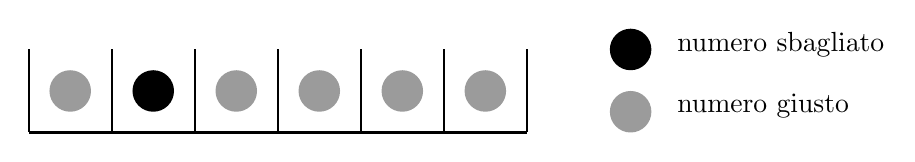
\begin{tikzpicture}[x=0.75pt,y=0.75pt,yscale=-1,xscale=1]
	%uncomment if require: \path (0,77); %set diagram left start at 0, and has height of 77

	%Straight Lines [id:da09449098783720666] 
	\draw    (50,60) -- (290,60) ;
	%Shape: Circle [id:dp40594633380564016] 
	\draw  [draw opacity=0][fill={rgb, 255:red, 155; green, 155; blue, 155 }  ,fill opacity=1 ] (60,40) .. controls (60,34.48) and (64.48,30) .. (70,30) .. controls (75.52,30) and (80,34.48) .. (80,40) .. controls (80,45.52) and (75.52,50) .. (70,50) .. controls (64.48,50) and (60,45.52) .. (60,40) -- cycle ;
	%Shape: Circle [id:dp6641428274341103] 
	\draw  [draw opacity=0][fill={rgb, 255:red, 0; green, 0; blue, 0 }  ,fill opacity=1 ] (100,40) .. controls (100,34.48) and (104.48,30) .. (110,30) .. controls (115.52,30) and (120,34.48) .. (120,40) .. controls (120,45.52) and (115.52,50) .. (110,50) .. controls (104.48,50) and (100,45.52) .. (100,40) -- cycle ;
	%Shape: Circle [id:dp7905252015750659] 
	\draw  [draw opacity=0][fill={rgb, 255:red, 155; green, 155; blue, 155 }  ,fill opacity=1 ] (140,40) .. controls (140,34.48) and (144.48,30) .. (150,30) .. controls (155.52,30) and (160,34.48) .. (160,40) .. controls (160,45.52) and (155.52,50) .. (150,50) .. controls (144.48,50) and (140,45.52) .. (140,40) -- cycle ;
	%Shape: Circle [id:dp33901503243236997] 
	\draw  [draw opacity=0][fill={rgb, 255:red, 155; green, 155; blue, 155 }  ,fill opacity=1 ] (180,40) .. controls (180,34.48) and (184.48,30) .. (190,30) .. controls (195.52,30) and (200,34.48) .. (200,40) .. controls (200,45.52) and (195.52,50) .. (190,50) .. controls (184.48,50) and (180,45.52) .. (180,40) -- cycle ;
	%Shape: Circle [id:dp9005911918848624] 
	\draw  [draw opacity=0][fill={rgb, 255:red, 155; green, 155; blue, 155 }  ,fill opacity=1 ] (220,40) .. controls (220,34.48) and (224.48,30) .. (230,30) .. controls (235.52,30) and (240,34.48) .. (240,40) .. controls (240,45.52) and (235.52,50) .. (230,50) .. controls (224.48,50) and (220,45.52) .. (220,40) -- cycle ;
	%Shape: Circle [id:dp4207926820924768] 
	\draw  [draw opacity=0][fill={rgb, 255:red, 155; green, 155; blue, 155 }  ,fill opacity=1 ] (260,40) .. controls (260,34.48) and (264.48,30) .. (270,30) .. controls (275.52,30) and (280,34.48) .. (280,40) .. controls (280,45.52) and (275.52,50) .. (270,50) .. controls (264.48,50) and (260,45.52) .. (260,40) -- cycle ;
	%Straight Lines [id:da9159657244031865] 
	\draw    (50,20) -- (50,60) ;
	%Straight Lines [id:da7573967278607023] 
	\draw    (90,20) -- (90,60) ;
	%Straight Lines [id:da7463985181158719] 
	\draw    (130,20) -- (130,60) ;
	%Straight Lines [id:da9290196388669603] 
	\draw    (170,20) -- (170,60) ;
	%Straight Lines [id:da06680789769911977] 
	\draw    (210,20) -- (210,60) ;
	%Straight Lines [id:da40034730485648806] 
	\draw    (250,20) -- (250,60) ;
	%Straight Lines [id:da4056303578838951] 
	\draw    (290,20) -- (290,60) ;
	%Shape: Circle [id:dp8217285666442] 
	\draw  [draw opacity=0][fill={rgb, 255:red, 0; green, 0; blue, 0 }  ,fill opacity=1 ] (330,20) .. controls (330,14.48) and (334.48,10) .. (340,10) .. controls (345.52,10) and (350,14.48) .. (350,20) .. controls (350,25.52) and (345.52,30) .. (340,30) .. controls (334.48,30) and (330,25.52) .. (330,20) -- cycle ;
	%Shape: Circle [id:dp043484895799565715] 
	\draw  [draw opacity=0][fill={rgb, 255:red, 155; green, 155; blue, 155 }  ,fill opacity=1 ] (330,50) .. controls (330,44.48) and (334.48,40) .. (340,40) .. controls (345.52,40) and (350,44.48) .. (350,50) .. controls (350,55.52) and (345.52,60) .. (340,60) .. controls (334.48,60) and (330,55.52) .. (330,50) -- cycle ;

	% Text Node
	\draw (361,10) node [anchor=north west][inner sep=0.75pt]   [align=left] {numero sbagliato};
	% Text Node
	\draw (361,40) node [anchor=north west][inner sep=0.75pt]   [align=left] {numero giusto};

	\end{tikzpicture}

	Il numero sbagliato può essere uno qualsiasi dei $6$ numeri che ho scelto, quindi ho $6$ modi possibili di sostituire il jolly al numero sbagliato.
	\item L'evento è dato dall'unione disgiunta:
	\begin{equation*}
		A\cup B\implies \PP(A\cup B) =\PP(A) +\PP(B) =\frac{7}{\binom{90}{6}} \approx 1.12\times 10^{-8}
	\end{equation*}
\end{enumerate}

\Soluzione

Poiché \textit{distinti}, possiamo enumerare gli oggetti dell'urna da $1$ a $n$. Introduciamo gli eventi $A_{j}^{m} =$ \event{esce l'oggetto $m$ all'estrazione $j$}:
\begin{equation*}
	A_{j}^{m} =\{\omega =(\omega_{1} ,\dots ,\omega_{k}) \in \Omega :\omega_{j} =m\} ,\ \ \ \ m\in \{1,\dots,n\} ,\ \ \ \ j\in \{1,\dots,k\}
\end{equation*}
\begin{enumerate}
	\item 
	\begin{enumerate}
		\item $\Omega $ è lo spazio campionario delle disposizioni \textit{con} ripetizione:
		\begin{align*}
			\Omega  & =\{1,\dots,n\}^{k}\\
			 & =\{\omega =(\omega_{1} ,\dots ,\omega_{k}) \in \Omega :\omega_{i} \in \{1,\dots,n\} ,i\in \{i,\dots,k\}\}\\
			 & \implies | \Omega | =n^{k}
		\end{align*}
		\item $(\impliedby)$ Ipotesi:
		\begin{enumerate}
			\item le $k$ estrazioni sono indipendenti, i.e.
			\begin{equation*}
				\PP\left(\bigcap_{j=1}^{k} A_{j}^{\omega_{j}}\right) =\prod_{j=1}^{k}\PP\left(A_{j}^{\omega_{j}}\right)
			\end{equation*}
			\item per ciascuna estrazione gli $n$ risultati possibili sono equiprobabili, i.e.
			\begin{equation*}
				\PP\left(A_{j}^{m}\right) =1/n\ \ \ \ \forall m,\forall j
			\end{equation*}
		\end{enumerate}
		Tesi da dimostrare: $\PP(\{\omega \}) =\frac{1}{| \Omega | } =\frac{1}{n^{k}} ,\forall \omega \in \Omega $.

		Abbiamo visto che i possibili evento $\omega \in \Omega $ sono della forma $\omega =(\omega_{1} ,\dots ,\omega_{k})$ con $\omega_{i} \in \{1,\dots,n\}$ e $i\in \{1,\dots,k\}$, allora
		\begin{align*}
			\PP(\{\omega \}) & =\PP(\{(\omega_{1} ,\dots ,\omega_{k})\}) & \\
			 & =\PP\left(\bigcap_{j=1}^{k} A_{j}^{\omega_{j}}\right) & \text{significato di} \ \omega \\
			 & =\prod_{j=1}^{k}\PP\left(A_{j}^{\omega_{j}}\right) & \text{indipendenza}\\
			 & =\prod_{j=1}^{k}\frac{1}{n} & \text{estrazioni equiprobabili}\\
			 & =\frac{1}{n^{k}} =\frac{1}{| \Omega | } & 
		\end{align*}

		$(\implies)$ esercizio.
		\item Sia $A=$ \event{estraggo gli oggetti $\{x_{1},\dots,x_{k}\}$ senza riguardo per l'ordine}. Dato che abbiamo la possibilità di ripetizioni, i casi possibili oscillano tra due estremi:
		\begin{enumerate}
			\item $\{x_{1},\dots,x_{k}\}$ è composto da oggetti tutti uguali: no permutazioni! (o meglio permutazioni di $k$ oggetti indistinguibili) $k!/k!=1$ possibilità. Quindi $| A| =1$.
			\item $\{x_{1},\dots,x_{k}\}$ è composto da oggetti tutti distinti: dato che non teniamo conto dell'ordine, dobbiamo tenere conto di tutte le possibili permutazioni. Quindi $| A| =k!$.
		\end{enumerate}

		Pertanto, $\frac{1}{n^{k}} \leq \PP(A) \leq \frac{k!}{n^{k}}$, nel \textit{mezzo} ci sono i casi con sottoclassi di oggetti uguali tra loro.
	\end{enumerate}
	\item 
	\begin{enumerate}
		\item $\Omega $ è lo spazio campionario delle disposizioni \textit{senza} ripetizione:
		\begin{align*}
			\Omega = & \{\omega =(\omega_{1} ,\dots ,\omega_{k}) \in \Omega :\omega_{i} \in \{1,\dots,n\} ,i\in \{i,\dots,k\}\\
			 & \ \ \ \ \omega_{i} \neq \omega_{j} \ \forall i\neq j\}\\
			\implies  & | \Omega | =n(n-1) \cdots (n-k+1) =\frac{n!}{(n-k) !}
		\end{align*}
		\item $(\implies)$ Analogamente al caso $1$, dobbiamo provare che
		\begin{equation*}
			\forall \omega \in \Omega \ \ \ \ \PP(\omega) =\frac{1}{| \Omega | } =\frac{1}{n(n-1) \cdots (n-k+1)}
		\end{equation*}

		Per ipotesi, sappiamo che ogni esito di ciascuna estrazione è equiprobabile \textit{condizionatamente} rispetto ai risultati delle passate estrazioni. Sfruttiamo il seguente risultato teorico \textit{(J.P. 3.3)} che connette indipendenza con probabilità condizionata per un numero finito di eventi.

		Sia $(\Omega ,\mathcal{A} ,\PP)$ uno spazio di probabilità e siano $A_{1} ,\dots ,A_{n} \in \mathcal{A}$ tale che $\PP(A_{1} \cap A_{2} \cap \cdots \cap A_{n-1})  >0$. Allora $\PP\left(\bigcap_{n} A_{n}\right) =\PP(A_{1})\PP(A_{2} |A_{1}) \cdots \PP(A_{n} |A_{1} \cap \cdots \cap A_{n-1})$.

		\begin{oss}
			Questo è esattamente il caso che ci interessa, perché quando estraiamo la $k$-esima pallina dobbiamo tenere conto del fatto che ne abbiamo estratte $k-1$ prima. Abbiamo allora:
			\begin{align*}
				\PP(\{\omega \}) & =\PP(\{\omega_{1} ,\dots ,\omega_{k}\})\\
				 & =\PP\left(\bigcap_{j=1}^{k} A_{j}^{\omega_{k}}\right)\\
				 & =\PP\left(A_{1}^{\omega_{1}}\right)\PP\left(A_{2}^{\omega_{2}} |A_{1}^{\omega_{1}}\right) \cdots \PP\left(A_{k}^{\omega_{k}} |A_{1}^{\omega_{1}} \cap \cdots \cap A_{k-1}^{\omega_{k-1}}\right)\\
				 & =\frac{\left| A_{1}^{\omega_{1}}\right| }{| \Omega | }\frac{\left| A_{2}^{\omega_{2}} \cap A_{1}^{\omega_{1}}\right| }{\left| A_{1}^{\omega_{1}}\right| } \cdots \frac{| A_{k}^{\omega_{k}} \cap \cdots \cap A_{1}^{\omega_{1}} |}{\left| A_{k-1}^{\omega_{k-1}} \cap \cdots \cap A_{1}^{\omega_{1}}\right| }\\
				 & =\frac{1}{n} \ \frac{1}{n-1} \cdots \frac{1}{n-(k-1)}\\
				 & =\frac{1}{n(n-1) \cdots (n-k+1)} =\frac{1}{| \Omega | }
			\end{align*}
		\end{oss}

		$(\impliedby)$ Esercizio.
		\item Sia $A$ come nel primo punto. Non abbiamo ripetizioni, perché stiamo considerando estrazioni senza reimmissione, dunque
		\begin{equation*}
			| A| =k!,\ \ \ \ \PP(A) =\frac{| A| }{| \Omega | } =\frac{k!(n-k) !}{n!} =\frac{1}{\binom{n}{k}}
		\end{equation*}
	\end{enumerate}
	\item 
	\begin{enumerate}
		\item $\Omega $ è lo spazio campionario delle combinazioni
		\begin{equation*}
			\Omega =\{\omega \subset \{1,\dots ,n\} :| \omega | =k\} ,\ \ \ \ | \Omega | =\binom{n}{k}
		\end{equation*}
		\item Sia $A$ come sopra, allora deve essere $\PP(A) =\frac{1}{\binom{n}{k}}$.
	\end{enumerate}
\end{enumerate}

\textbf{Osservazioni.}
\begin{itemize}
	\item Deve risultare che le probabilità $\PP(A)$ dei punti $2c$ e $3b$ siano uguali (confronta con es $3b$ e es $9a$ [OSS]).
	\item Importanza di questo esercizio.
	\begin{itemize}
		\item Serve per capire quando la probabilità uniforme è il modello corretto.
		\item La probabilità uniforme \textit{dipende} da $\Omega $, confronta punti $1b$ e $2b$.
	\end{itemize}
\end{itemize}

\Soluzione

\begin{equation*}
	\begin{drcases}
		7\ \text{blu}\\
		3\ \text{rosse}
	\end{drcases}
	\ 10\ \text{palline}\rightarrow \text{ne estraggo} \ 4
\end{equation*}
\begin{enumerate}
	\item \textit{Estrazione con reimmissione.}

	In questo caso abbiamo:
	\begin{equation*}
	\Omega =\{(\omega_{1} ,\dots ,\omega_{4}) :\omega_{i} \in \{1,\dots ,10\}\}
	\end{equation*}

	Spazio campionario delle disposizioni con ripetizione
	\begin{equation*}
	| \Omega | =10^{4}
	\end{equation*}

	Sia $A$ l'evento "$2$ palline rosse su $4$ estratte". Quanti modi ho di estrarre $2$ palline rosse e $2$ blu? Ho $3^{2} \cdot 7^{2}$ possibilità di scelta, ma poi dobbiamo considerare tutte le possibili permutazioni $\binom{4}{2} =\frac{4!}{2!2!}$.
	\begin{equation*}
		\implies | A| =\binom{4}{2} 3^{2} 7^{2}\implies \PP(A) =\frac{| A| }{| \Omega | } =\binom{4}{2}\frac{3^{2} 7^{2}}{10^{4}} \approx 0.2646.
	\end{equation*}
	\item \textit{Estrazione senza reimmissione.}

	Svolgiamo l'esercizio in due diversi modi, introducendo $\Omega $ in due diversi modi.
	\begin{enumerate}
		\item Metodo $1$
		\begin{equation*}
			\Omega =\{(\omega_{1} ,\dots ,\omega_{4}) :\omega_{i} \in \{1,\dots ,10\} ,\omega_{i} \neq \omega_{j} \ \forall i\neq j\}
		\end{equation*}

		Spazio campionario delle disposizioni senza ripetizione
		\begin{equation*}
			| \Omega | =10\cdot 9\cdot 8\cdot 7=\frac{10!}{6!}
		\end{equation*}

		Sia $A$ l'evento "$2$ palline rosse su $4$ estratte". Quanti modi abbiamo di estrarre $2$ palline rosse e $2$ blue? In totale abbiamo $(3\cdot 2) \cdot (7\cdot 6)$ possibilità di ottenere questa configurazione, però dobbiamo considerare tutti i possibili modi in cui le $2$ palline rosse possono disporsi su $4$ ($=$ palline estratte) posti i.e. dobbiamo considerare tutte le $\binom{4}{2}$ possibili configurazioni.

		\begin{oss}
			Possiamo pensare anche pensare il tutto come il modo di permutare le $4$ palline, tenendo conto che $2$ rosse sono indistinguibili e $2$ blu sono indistinguibili.
			\begin{gather*}
				\binom{4}{2} =\frac{4!}{2!2!} =\frac{4\cdot 3\cdot 2}{4} =6\ \text{possibili modi}\\
				\Downarrow \\
				| A| =\binom{4}{2} \cdot (3\cdot 2) \cdot (7\cdot 6)\\
				\PP A) =\frac{| A| }{| \Omega | } =\frac{\binom{4}{2} \cdot (3\cdot 2) \cdot (7\cdot 6)}{10\cdot 9\cdot 8\cdot 7} \approx 0.3
			\end{gather*}
		\end{oss}

		\item Metodo $2$
		\begin{equation*}
			\Omega =\{\omega \subset \{1,\dots ,10\} \ |\ | \omega | =4\}
		\end{equation*}
		Spazio campionario delle combinazioni
		\begin{equation*}
			| \Omega | =\binom{10}{4}
		\end{equation*}
		Sia $A$ l'evento "$2$ palline rosse su $4$ estratte". Quanti modi ho di estrarre $2$ palline rosse e $2$ blu? Abbiamo
		\begin{gather*}
			\binom{3}{2} \ \text{modi di scegliere le palline rosse}\\
			\binom{7}{2} \ \text{modi di scegliere le palline blu}\\
			\implies | A| =\binom{3}{2}\binom{7}{2}\\
			\PP(A) =\frac{| A| }{| \Omega | } =\frac{\binom{3}{2}\binom{7}{2}}{\binom{10}{4}} \approx 0.3
		\end{gather*}
	\end{enumerate}
	\item \textit{Estrazione simultanea}

	Questo caso si tratta esattamente come il metodo $2$ del punto precedente.
\end{enumerate}

\Soluzione

Manca.

\Soluzione

Manca.

\Soluzione

Manca.

\Soluzione

Manca.

\Soluzione

Manca.

\Soluzione

Introduciamo $\Omega $ come lo spazio delle combinazioni di $52$ elementi di classe $5$, i.e.
\begin{equation*}
	\Omega =\{\omega \subset \{1,\dots ,52\} \ |\ | \omega | =5\} ,\ \ \ \ | \Omega | =\binom{52}{5}
\end{equation*}
\begin{enumerate}
	\item Sia $A$ l'evento "esce un full" (esempio di full: $3\varheartsuit \ 3\spadesuit \ 3\vardiamondsuit \ 6\varheartsuit \ 6\clubsuit $)\begin{equation*}
	| A| =13\cdot \binom{4}{3} \cdot 12\cdot \binom{4}{2}
	\end{equation*}
	\begin{enumerate}
		\item ho $13$ possibilità per scegliere il tipo del tris (es. scelgo il $3$)
		\item ho $\binom{4}{3}$ possibilità di scegliere il seme (posso pensarlo come ad un'urna in cui ho $4$ semi e ne estraggo $3$, es. estratto $\varheartsuit ,\spadesuit ,\vardiamondsuit $)
		\item ho $12$ possibilità per scegliere il tipo della coppia (es. scelgo il $6$)

		\begin{oss}
			In questo caso considero $13\cdot 12$ possibilità per il tipo e NON $\binom{13}{2}$ perché i casi $(3\varheartsuit \ 3\spadesuit \ 3\vardiamondsuit \ 6\varheartsuit \ 6\clubsuit) \neq (6\varheartsuit \ 6\spadesuit \ 6\vardiamondsuit \ 3\varheartsuit \ 3\clubsuit)$, differenza con il punto successivo
		\end{oss}

		\item ho $\binom{4}{2}$ possibilità di scegliere il seme (es. $\varheartsuit ,\clubsuit $)
		\begin{equation*}
			\implies \PP(A) =\frac{| A| }{| \Omega | } =\frac{13\cdot \binom{4}{3} \cdot 12\cdot \binom{4}{2}}{\binom{52}{5}} \approx 0.0014
		\end{equation*}
	\end{enumerate}
	\item Sia $B$ l'evento "esce una doppia coppia" (esempio di doppia coppia: $3\varheartsuit \ 3\vardiamondsuit \ 7\clubsuit \ 7\varheartsuit \ 11\spadesuit $)
	\begin{equation*}
		| B| =\binom{13}{2}\binom{4}{2}\binom{4}{2} \cdot 11\cdot 4
	\end{equation*}
	\begin{enumerate}
		\item ho $\binom{13}{2}$ modi per scegliere i due tipi (es. escono il $3$ e il $7$)
		\item ho $\binom{4}{2}$ modi di scegliere i semi per la prima coppia
		\item ho $\binom{4}{2}$ modi di scegliere i semi per la seconda coppia
		\item mi rimangono $11$ possibilità tra cui scegliere il \textit{numero/figura} dell'ultima carta
		\item posso scegliere uno qualunque dei $4$ semi possibili per l'ultima carta
		\begin{equation*}
			\implies \PP(B) =\frac{| B| }{| \Omega | } =\frac{\binom{13}{2}\binom{4}{2}\binom{4}{2} \cdot 11\cdot 4}{\binom{52}{5}} \approx 0.0475
		\end{equation*}
	\end{enumerate}
	\item [punto e] Sia $C$ l'evento "esce una scala".
	\begin{gather*}
		| C| =10\cdot 4^{5}\\
		A\ 2\ 3\ 4\ 5\ 6\ 7\ 8\ 9\ 10\ |\ J\ Q\ K
	\end{gather*}
	\begin{enumerate}
		\item $10$ possibilità $\rightarrow $ blocco la prima carta: ho $10$ possibilità, non posso far partire la scala da $J,Q,K$.
		\item per ogni carta ho $4$ possibilità sui semi
		\begin{equation*}
			\implies \PP(C) =\frac{| C| }{| \Omega | } =\frac{10\cdot 4^{5}}{\binom{52}{5}}
		\end{equation*}
	\end{enumerate}
	\item [punto h] Sia $D$ l'evento "esce un tris" (esempio di tris: $3\varheartsuit \ 3\vardiamondsuit \ 3\spadesuit \ 4\vardiamondsuit \ 5\varheartsuit $)
	\begin{equation*}
		| D| =13\cdot \binom{4}{3} \cdot \binom{12}{2} \cdot 4\cdot 4
	\end{equation*}
	\begin{enumerate}
		\item ho $13$ possibilità per il tipo del tris (es. esce il $3$)
		\item ho $\binom{4}{3}$ possibilità per scegliere il seme del tris
		\item ho $\binom{12}{2}$ possibilità per scegliere il tipo delle altre carte
		\item ho $4$ possibilità per scegliere il seme della quarta e della quinta carta
		\begin{equation*}
			\implies \PP(D) =\frac{| D| }{| \Omega | } =\frac{13\cdot \binom{4}{3} \cdot \binom{12}{2} \cdot 4\cdot 4}{\binom{52}{5}}
		\end{equation*}
	\end{enumerate}
\end{enumerate}